\section{Introduction, scope, and process taxonomy}
\label{sec:introduction}
\subsection{The manufacturing question}
The useful question is not simply whether glass can be printed. It is whether a specified composition can be formed into an accepted geometry, at a repeatable rate, with the required optical, mechanical, thermal, and chemical properties. A transparent sculpture, a microfluidic channel, and a load-bearing glass connection place very different demands on the process. This report centers on direct deposition of hot inorganic glass and uses other additive routes as explicitly identified comparators.

The strongest case for additive manufacturing is geometric customization that is expensive or impractical with a repeated mold or accessible machining surface. Eliminating a mold does not eliminate conditioning, finishing, thermal treatment, or inspection. Conversely, accepting the native layer texture can create useful optical and aesthetic functions. Decisions should therefore begin with a part specification and a conventional-process baseline, not an assumption that additive manufacture is preferable.

\subsection{A taxonomy by material state and consolidation step}
\textbf{Reservoir-fed molten extrusion} conditions a quantity of glass in a crucible and deposits it through a heated nozzle. Gravity, imposed pressure, or mechanical metering drives flow. The receiving chamber manages cooling while a motion system lays down a continuous cord. Early G3DP and G3DP2 are reference demonstrations of this family.\cite{acad_klein2015,acad_inamura2018}

\textbf{Locally heated solid-feed deposition} delivers a glass rod or filament to a hot zone. A furnace-like nozzle or a laser heats only the material needed for deposition. Laser filament systems are particularly relevant to fused silica, whose viscosity at the same temperature differs greatly from soda-lime compositions. This route is analogous in material delivery to wire-fed directed-energy deposition, but it requires glass-specific treatment of optical absorption and stress.\cite{acad_liu2022}

\textbf{Powder-bed fusion} scans successive powder layers with a heat source. Packing, absorption, track consolidation, residual porosity, and cracking become central variables. Laser scan speed is not a net part-production rate: powder recoating, track overlap, contour passes, and rejected builds must be included. The labels SLS and SLM in the glass literature should be interpreted from the actual consolidation mechanism rather than treated as proof of complete densification.\cite{phys_datsiou}

\textbf{Indirect printing and conversion} shapes silica-containing inks, photopolymer nanocomposites, or precursors before drying, debinding, and densification. Stereolithography, two-photon polymerization, direct ink writing, and computed axial lithography belong here when the printed object is a precursor rather than final dense glass. The printing temperature can be near room temperature while subsequent firing is much hotter. Kotz and colleagues demonstrated transparent fused-silica structures by photopolymerizing a nanocomposite and heat treating it; Toombs and colleagues demonstrated volumetric shaping followed by sintering.\cite{phys_kotz,phys_toombs}

These routes exclude glass-fiber-filled thermoplastics, sugar glass, and metallic glasses from the core comparison. Chalcogenide glass extrusion is considered in the academic directory as a distinct material family, not as evidence for the same silicate processing window. Additively manufacturing a metal mold used to form glass is also an adjacent tooling route rather than direct glass printing.

\subsection{Evidence selection and reproducibility}
Source discovery covered primary journal articles, institutional repositories, manufacturer technical documents, institutional project pages, and patent records. DOI metadata were collected from Crossref where accessible; downloaded PDFs were parsed and retained with provenance. Reviews informed discovery but did not substitute for primary apparatus or property evidence. Institutional and manufacturer pages establish reported activity or supplier claims, not independently audited performance.

The companion source index and manifest retain individual records, retrieval dates, local paths, and asset hashes. Different versions of a supplier page were encountered during research; current certified ratings were not inferred from an older cached specification. Where a paper or site was blocked, the report identifies the narrower evidence actually available. This search did not enumerate every indexed paper or conduct a formal study-quality meta-analysis. Coverage of named institutions is an evidence map, including explicit negative search outcomes, rather than proof of their current equipment inventories.

Table~\ref{tab:routes} is deliberately a comparison of documented examples. It is not a normalized benchmark. NR means that the cited evidence does not establish a comparable numerical value; it does not mean zero or poor performance. Relative tensile strength is particularly unsuitable for inference from bend tests performed on different compositions and flaw populations.

\begin{table}[htbp]
\centering\small
\caption{Direct molten extrusion versus powder-bed fusion and photopolymer/sintering routes. Temperatures and rates refer to the indicated examples, not universal or certified machine limits.}
\label{tab:routes}
\begin{tabularx}{\textwidth}{@{}P{0.17\textwidth}YYY@{}}
\toprule
Metric & Molten reservoir extrusion & Glass laser powder-bed fusion & Photopolymer shaping + sintering \\
\midrule
Representative evidence & G3DP2, 2018 \cite{acad_inamura2018} & Soda-lime LPBF, 2019 \cite{phys_datsiou} & Fused-silica SLA, 2017; micro-CAL, 2022 \cite{phys_kotz,phys_toombs} \\
Temperature ($^{\circ}$C) & Reservoir operating 1090; separate delivery/build zones & Local transient melt temperature NR; 1280 is the paper's material thermal-characterization value, not a measured laser-pool setpoint & Near-ambient shaping; formulation-specific high-temperature densification. UpQuartz example: 1300 sintering \cite{com_upnano} \\
Build envelope & G3DP2: $320\times320\times350$ mm; earlier G3DP: $250\times250\times300$ mm (source Table~1) & Comparable validated maximum NR & Comparable validated maximum NR; demonstrated microstructures are not machine envelope \\
Deposition rate & G3DP2: 5.2 kg/h $\approx86.7$ g/min; deposited flow, excludes annealing & Net accepted-part rate NR & Net glass volume/time NR; micro-CAL exposure 30--90 s excludes subsequent firing \\
Optical transmission $T\%$ & Transparent demonstrators; comparable spectral $T\%$ NR & Opaque as-built examples; comparable spectral $T\%$ NR & Transparent fused silica reported; comparable thickness/wavelength-normalized $T\%$ NR \\
Surface roughness $R_a$ & Comparable quantified $R_a$ NR; bead texture retained & Comparable quantified $R_a$ NR; partially fused surface particles & Micro-CAL sintered lens: $R_a=60$ nm over 523 $\mu$m; 6 nm over 49 $\mu$m (source Fig.~S17); not a whole-part specification \\
Relative tensile strength & NR: bending/structural tests cannot establish a universal tensile ratio & NR & NR: specimen type and loading differ \\
\bottomrule
\end{tabularx}
\end{table}

The G3DP2 paper reports both 570 mm$^3$/s and 5.2 kg/h as rounded production descriptors; neither includes a complete end-to-end production cycle. Its comparison to earlier platforms should not be extended to every modern indirect printer. The LPBF study reported approximately 11--12\% internal porosity in selected specimens and observed improved translucency with a subsequent 650~$^{\circ}$C heat treatment. Those findings concern one powder and processing window, not an upper bound on all powder-bed glass methods.\cite{acad_inamura2018,phys_datsiou}

\begin{figure}[htbp]
\centering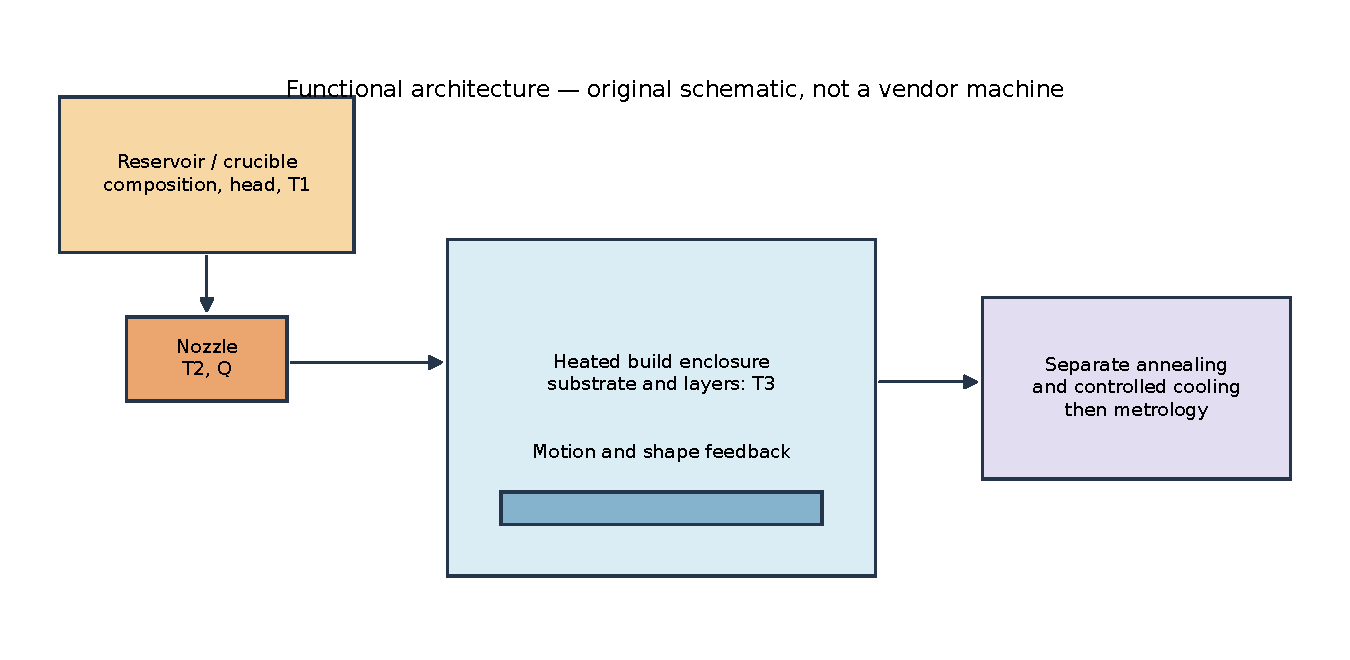
\includegraphics[width=\linewidth]{figures/process_architecture.pdf}
\caption{Original functional schematic separating reservoir conditioning, delivery, receiving environment, and downstream annealing. It describes engineering functions, not the construction or specification of a particular commercial printer.}
\label{fig:architecture}
\end{figure}
